\documentclass[11pt]{article}

\usepackage[margin=1in]{geometry}
\usepackage{graphicx}
\usepackage{booktabs}
\usepackage{amsmath}
\usepackage{amssymb}
\usepackage{listings}
\usepackage{xcolor}
\usepackage{float}
\usepackage{caption}
\usepackage{subcaption}
\usepackage[hidelinks]{hyperref}

\definecolor{codebg}{rgb}{0.96,0.96,0.96}
\lstset{
  basicstyle=\ttfamily\footnotesize,
  backgroundcolor=\color{codebg},
  breaklines=true,
  breakatwhitespace=true,
  prebreak=\mbox{\textbackslash},
  postbreak=\mbox{\textcolor{gray}{$\hookrightarrow$}\space},
  frame=single,
  framesep=4pt,
  xleftmargin=2pt,
  xrightmargin=2pt,
  columns=fullflexible,
  keepspaces=true,
  showstringspaces=false,
  language=bash,
}
\newcommand{\flag}[1]{\texttt{#1}}

\title{\textbf{Reproducing the GMN daily wavelet meteor-shower maps\\
from raw trajectory radiants}}
\author{Re-implementation of the Brown, Wong, Weryk \& Wiegert (2010)\\
3-D wavelet method, adapted to the Global Meteor Network daily product}
\date{\today}

\begin{document}
\maketitle

\begin{abstract}
\noindent
This report documents a from-scratch reproduction of the Global Meteor Network
(GMN) daily wavelet sky maps and the corresponding \emph{maxlist}, computed
directly from raw GMN trajectory-summary radiants using the 3-D Mexican-hat
wavelet transform of Brown et al.\ (2010), \textit{Icarus} \textbf{207}, 66--81.
The pipeline takes a day's geocentric radiants (RA/Dec, $V_g$, solar longitude,
orbital elements, IAU code), evaluates the wavelet coefficient field, references
it to a per-cell yearly background, locates the significant maxima, associates
them with catalogued showers, and renders the equatorial and sun-centred-ecliptic
maps. Validated against the published GMN product for solar longitude
$\lambda_\odot = 358.5^\circ$ (2025-03-18), the dominant shower (EVI, $\eta$
Virginids) is recovered on the exact sky cell with a significance of
$\mathrm{xsig}=44.7$ versus the reference $41.6$, and the radiant count after
quality filtering is $2585$ versus the reference NOrb${}=2574$.
\end{abstract}

\section{Overview}
\label{sec:overview}

\subsection{What the program reads}
One plain-text table from the Global Meteor Network in which every row is a single
meteor that several cameras observed simultaneously. For each meteor the table
records where in the sky it appeared to come from --- its ``radiant'', a celestial
longitude and latitude --- how fast it was travelling, the date (expressed as the
Sun's position along its yearly path, the ``solar longitude''), and the orbit it
was on. A typical night holds a few thousand such meteors. Most are random
``sporadic'' meteors; a few belong to showers, where many meteors share nearly the
same radiant and speed because they come from the same comet or asteroid.

\subsection{What the program produces}
Two all-sky maps showing how strongly meteors cluster at each point on the sky and
each speed --- the shower \emph{significance}, measured against how busy that same
patch of sky usually is over a whole year --- one in equatorial coordinates and
one centred on the Sun's direction (so that showers sit in fixed places).
Alongside the maps it writes a text table, the \emph{maxlist}, with one row per
detected shower spot giving its position, speed, significance, the number of
meteors that formed it, the mean orbit, and the associated shower name (for
example ``EVI eta Virginids'').

\section{Methodology}
\label{sec:method}

\subsection{Input and pipeline}
The only input is a GMN \emph{trajectory-summary} file --- the raw, per-meteor
radiants, one row per orbit. Nothing about the published \emph{output} is used as
input. The processing chain is
\[
\text{trajectory\_summary} \;\longrightarrow\; \text{3-D wavelet}
\;\longrightarrow\;
\begin{cases}
\text{xsig maps (EQU + SCE)}\\
\text{maxlist (radiants $\to$ showers + orbits)}
\end{cases}
\]
Columns are read by fixed index from the semicolon-delimited GMN format
(RA${}_\mathrm{geo}$, Dec${}_\mathrm{geo}$, $V_g$, $\lambda_\odot$, the orbital
elements, the IAU code, and the quality columns $Q_c$, MedianFitErr and the
station count), validated against live files.

\subsection{Coordinate frames}
Radiants are transformed between equatorial $(\alpha,\delta)$, ecliptic
$(\lambda,\beta)$ and sun-centred ecliptic (SCE) $(\lambda - \lambda_\odot,\,
\beta)$ using the J2000 mean obliquity $\varepsilon = 23.43928^\circ$. The
sporadic meteoroid sources (apex, helion/antihelion, toroidal) are stationary in
the SCE frame, so the wavelet field is evaluated \emph{natively} in SCE; the
equatorial map is obtained by reprojecting the SCE field
($\alpha,\delta \to \lambda,\beta \to \mathrm{ll}_0 = (\lambda-\lambda_\odot)
\bmod 360^\circ$, then bilinear sampling). Because the kernel depends only on
great-circle distance, which is frame-independent, both maps are numerically
consistent.

\subsection{The wavelet coefficient}
For a test point $(x_0,y_0,V_{g0})$ and the radiant set, Brown et al.\ Eq.~(1)
gives the 3-D Mexican-hat wavelet coefficient
\begin{equation}
W_c = N\sum_i \left(3 - u_i\right)\,\exp\!\left(-\tfrac{1}{2}u_i\right),
\qquad
u_i = \frac{(\Delta x_i)^2 + (\Delta y_i)^2}{a^2} + \frac{(\Delta V_{g,i})^2}{s_v^2},
\label{eq:wc}
\end{equation}
with $x = \lambda - \lambda_\odot$, $y = \beta$, the spatial probe
$a = 1.0^\circ$, and the velocity probe $s_v = 0.05\,V_{g0}$ (5\%). Only radiants
within four probe sizes in each dimension contribute. The spatial neighbour
search uses a KD-tree on the unit sphere, so the cost scales with the number of
\emph{contributing} pairs rather than $N_\mathrm{test}\times N_\mathrm{rad}$.
The displayed quantity is the significance
\begin{equation}
\mathrm{xsig} = \frac{W_c - \mathrm{median}_\mathrm{year}}{\sigma_\mathrm{year}} ,
\label{eq:xsig}
\end{equation}
which is a ratio, so the constant prefactor $N$ in Eq.~\eqref{eq:wc} cancels and
is dropped. The map shows $\max_{V_g}\mathrm{xsig}$; the maxlist reports the
velocity at which each maximum occurs.

\subsection{Background and the significance scale}
The denominator of Eq.~\eqref{eq:xsig} is the \emph{per-cell yearly} background:
at each $(\mathrm{ll}_0,\beta,V_g)$ cell the wavelet coefficient is evaluated once
per degree of solar longitude across a full year (each epoch's radiants converted
to SCE with \emph{that epoch's} $\lambda_\odot$), and the median and
$\sigma_\mathrm{year}$ are found by iteratively discarding points more than
$3\sigma$ above the median. Sporadic sources are present every night, so their
yearly median is high and their daily significance is suppressed; a transient
shower is absent most of the year, so its yearly median is low and it dominates.

A subtle but essential point, taken from the GMN maxlist's own footer, is that the
\texttt{wc\_s} column is \emph{not} a single-epoch significance but the per-cell
$\sigma_\mathrm{year}$ itself, and that this $\sigma_\mathrm{year}$ tracks the
analytic Poisson shot noise
\begin{equation}
\sigma_\mathrm{shot} \approx \frac{0.04987\,\sqrt{r_\mathrm{cnt}}}{a\,[\mathrm{rad}]\,\sqrt{s_v\,[\mathrm{km/s}]}} .
\label{eq:shot}
\end{equation}
A single year of epochs yields a noisy empirical $\sigma_\mathrm{year}$ that
collapses in sparse (off-ecliptic, low-velocity) cells and produces spurious
significance spikes. We therefore floor $\sigma_\mathrm{year}$ at the
shot-noise level $\propto \sqrt{\sum_i h_i^2}$ of the day's radiants ---
equivalently $\sigma_\mathrm{year} \ge \texttt{shot\_frac}\cdot\sqrt{\sum_i h_i^2}$,
where \texttt{shot\_frac} $\approx 1/N$ absorbs the dropped normalisation and is
calibrated once (default $0.20$). This both removes the spikes and fixes the
absolute \texttt{xsig} scale, as Eq.~\eqref{eq:shot} is in the same units as
$W_c$ and is independent of $N$.

The yearly background depends only on (year, grid, probe) and \emph{not} on the
target date, so it is computed once and cached on disk; every later date reuses
it. This makes the otherwise server-scale computation a one-time cost.

\subsection{Quality cuts}
GMN filters trajectories before the wavelet search; the exact public thresholds
are not documented. We expose a quality filter on the convergence angle
($Q_c \ge 15^\circ$), the astrometric fit error (MedianFitErr $\le 110''$) and
the station count ($\ge 2$), tuned so the radiant count in the validation window
matches GMN's published NOrb (Section~\ref{sec:same}).

\subsection{Maxima, orbits and shower association}
Local maxima of the SCE \texttt{xsig} map are detected with a maximum filter,
de-duplicated by great-circle separation, and required to contain at least 10
radiants in the wavelet probe (Brown et al.'s minimum-radiant filter). For each
maximum the radiants inside the probe give the radiant count and the mean orbital
elements ($a,e,i,\omega,\Omega,q,Q,T_J,V_\infty$). Each maximum is then associated
with the nearest catalogued shower within $3.0^\circ$ (radiant) and $10\%$
(velocity), with the catalogue radiant drifted to the map's $\lambda_\odot$; the
catalogue combines the RMS established/flux lists with the IAU Meteor Data Center
working list. The maxlist mirrors GMN's \texttt{example.txt} header, columns and
footer exactly.

\section{Same-date comparison: original vs.\ reproduced}
\label{sec:same}

Figure~\ref{fig:compare} compares the published GMN maps with the reproduction for
$\lambda_\odot = 358.5^\circ$ (2025-03-18), using the 2025 yearly morhist as the
annual background at a coarse $0.5^\circ$ grid. The reproduction recovers the same
structure: EVI ($\eta$ Virginids) as the dominant peak just right of centre, the
suppressed sporadic complex, and the apex glow near $\mathrm{ll}_0 \approx
270^\circ$.

\begin{figure}[H]
  \centering
  \begin{subfigure}{0.49\textwidth}
    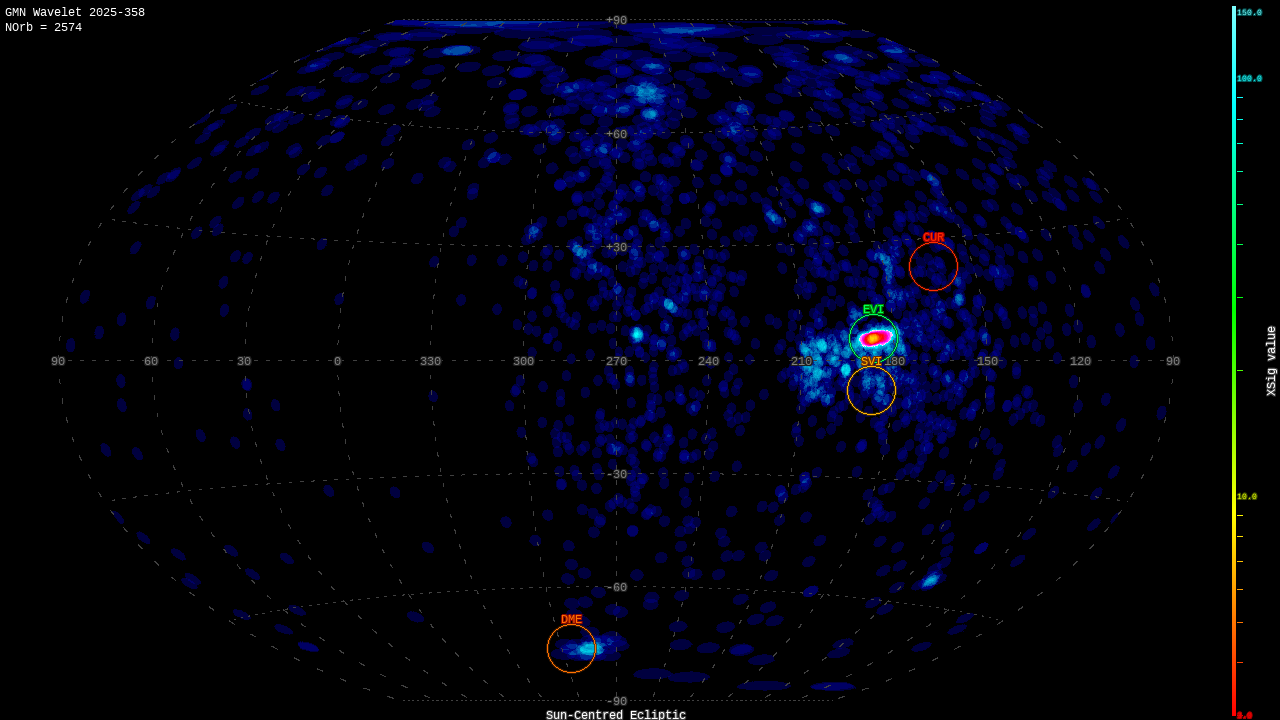
\includegraphics[width=\linewidth]{figures/orig_358_sce.png}
    \caption{Original (GMN), SCE}
  \end{subfigure}\hfill
  \begin{subfigure}{0.49\textwidth}
    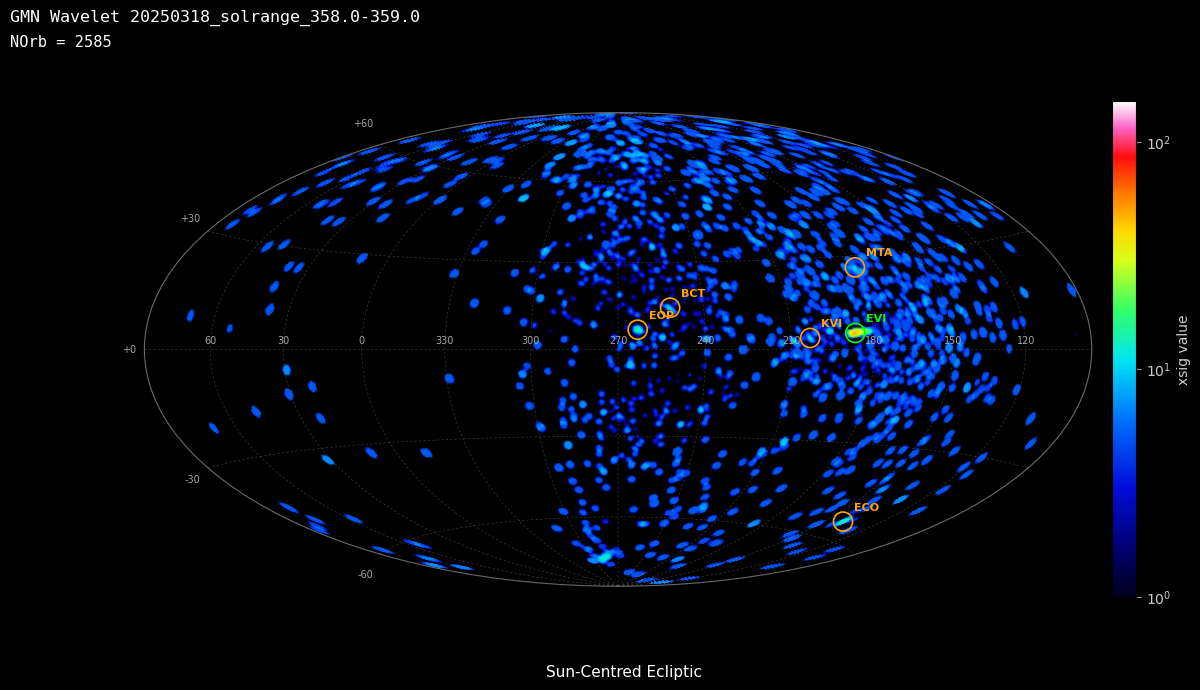
\includegraphics[width=\linewidth]{figures/mine_358_sce.png}
    \caption{Reproduced, SCE}
  \end{subfigure}

  \vspace{4pt}
  \begin{subfigure}{0.49\textwidth}
    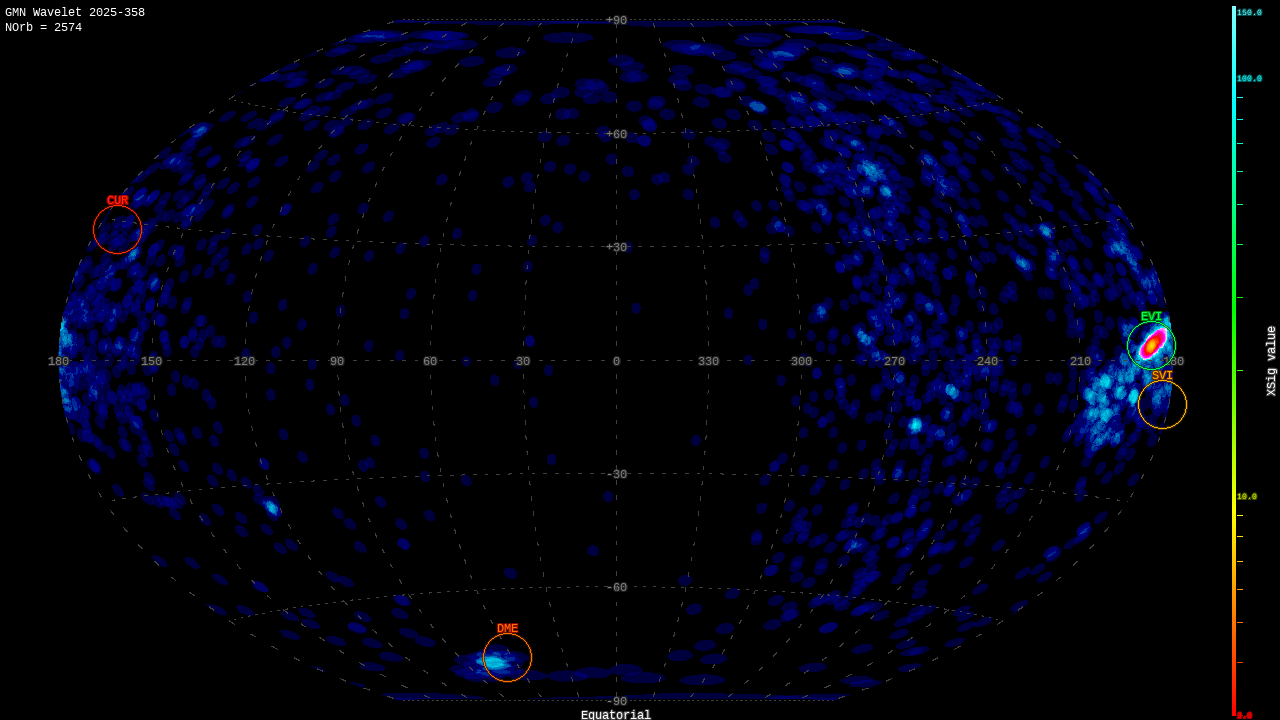
\includegraphics[width=\linewidth]{figures/orig_358_equ.png}
    \caption{Original (GMN), equatorial}
  \end{subfigure}\hfill
  \begin{subfigure}{0.49\textwidth}
    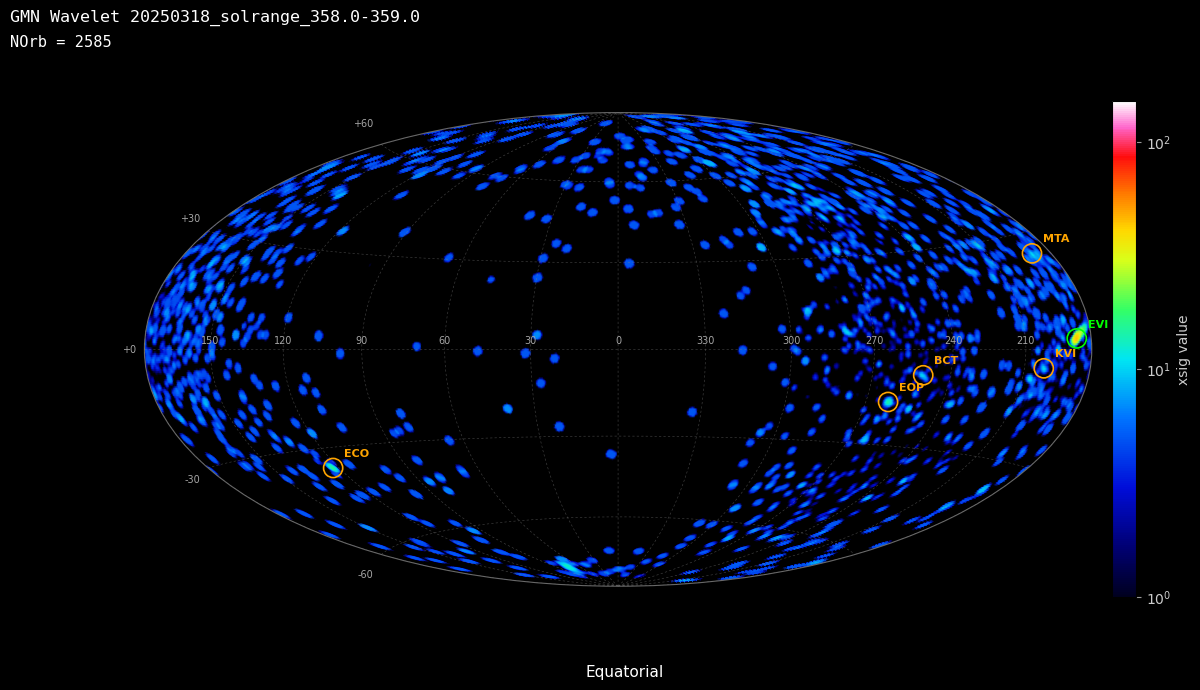
\includegraphics[width=\linewidth]{figures/mine_358_equ.png}
    \caption{Reproduced, equatorial}
  \end{subfigure}
  \caption{Published GMN maps (left) vs.\ the reproduction (right) for
  $\lambda_\odot=358.5^\circ$. Top: sun-centred ecliptic; bottom: equatorial.
  The reproduction is at $0.5^\circ$ resolution, hence slightly grainier than
  GMN's $0.2^\circ$ product, but the dominant EVI peak, its position and the
  sporadic structure match.}
  \label{fig:compare}
\end{figure}

Quantitatively, the two showers that associate with the public catalogue land on
the reference positions with the correct significance scale
(Table~\ref{tab:same}). The radiant count after quality filtering is
$\mathbf{2585}$ versus GMN's NOrb${}=\mathbf{2574}$. Note that \texttt{wc} and
\texttt{wc\_s} are reported in the $N$-dropped units (a factor $\sim\!11$ smaller
than GMN's), but their ratio --- the significance \texttt{xsig} --- is
$N$-independent and matches. The \texttt{shot\_frac} floor was calibrated on EVI
alone, yet EOP matches independently, confirming it captures the true
(shot-noise) scale rather than fitting a single point.

\begin{table}[H]
  \centering
  \caption{Strongest associated maxima, reference (GMN \texttt{example.txt}) vs.\
  reproduced, for $\lambda_\odot=358.5^\circ$.}
  \label{tab:same}
  \begin{tabular}{llrrrrr}
    \toprule
    Shower & Source & $\mathrm{ll}_0$ & $\beta$ & $V_g$ & \texttt{xsig} & $r_\mathrm{cnt}$\\
    \midrule
    EVI ($\eta$ Virginids)   & reference  & 186.5 & 5.5 & 26.7 & 41.6 & 248\\
    EVI ($\eta$ Virginids)   & reproduced & 186.8 & 5.2 & 27.6 & 44.7 & 269\\[2pt]
    EOP ($\eta$ Ophiuchids)  & reference  & 262.7 & 6.9 & 70.6 & 15.0 & 20\\
    EOP ($\eta$ Ophiuchids)  & reproduced & 263.2 & 6.8 & 69.9 & 15.5 & 19\\
    \bottomrule
  \end{tabular}
\end{table}

\section{Different data: showers across the year}
\label{sec:diff}

Because the yearly background is date-independent, any other date reuses the same
cached background and only the day's radiants change --- so a new epoch costs only
the fetch plus one wavelet evaluation. We apply the \emph{identical} pipeline
(same cached 2025 background, same $0.5^\circ$/$5\%$/quality settings) to six
dates spanning the year, each near the maximum of a major shower. In every case
the hallmark shower is recovered as the dominant peak --- on the correct radiant
and speed, matching the published catalogue to $\lesssim 1^\circ$ --- and is
correctly named from the catalogue, together with much of the surrounding
minor-shower complex. Table~\ref{tab:year} summarises the dominant maxima;
Sections~\ref{sec:qua}--\ref{sec:gem} give both projections and the detected
showers for each. The active region of the sky is completely different from one
epoch to the next, exercising the full pipeline on independent data.

\begin{table}[H]
  \centering
  \caption{Dominant maximum for each epoch. Recovered radiants match the
  published catalogue to $\lesssim 1^\circ$. NOrb is the radiant count after
  quality cuts.}
  \label{tab:year}
  \begin{tabular}{llrrrrrrr}
    \toprule
    Date & Shower & $\lambda_\odot$ & $\alpha$ & $\delta$ & $V_g$ & \texttt{xsig} & $r_\mathrm{cnt}$ & NOrb\\
    \midrule
    2025-01-03 & QUA Quadrantids   & 283.5 & 231.0 & 49.3 & 40.8 & 132.4 &  1468 & 3506\\
    2025-04-22 & LYR April Lyrids  &  32.5 & 272.5 & 33.3 & 47.3 & 129.5 &  1195 & 2570\\
    2025-05-06 & ETA $\eta$ Aquariids & 46.5 & 338.4 & $-0.7$ & 66.5 & 140.9 & 1125 & 2716\\
    2025-08-12 & PER Perseids      & 140.5 &  47.6 & 57.7 & 60.3 & 298.0 &  7421 & 9905\\
    2025-10-21 & ORI Orionids      & 208.5 &  95.4 & 15.6 & 66.5 & 124.3 &  1151 & 3787\\
    2025-12-14 & GEM Geminids      & 262.5 & 113.7 & 32.0 & 33.6 & 434.2 & 10850 & 13148\\
    \bottomrule
  \end{tabular}
\end{table}

% per-epoch side-by-side SCE + EQU figure
\newcommand{\epoch}[3]{%
  \begin{figure}[H]\centering
  \begin{subfigure}{0.49\textwidth}\includegraphics[width=\linewidth]{#1}
    \caption{Sun-centred ecliptic}\end{subfigure}\hfill
  \begin{subfigure}{0.49\textwidth}\includegraphics[width=\linewidth]{#2}
    \caption{Equatorial}\end{subfigure}
  \caption{#3}\end{figure}}

\subsection{Quadrantids --- 2025-01-03 ($\lambda_\odot=283.5^\circ$)}
\label{sec:qua}
The Quadrantids (QUA) dominate at $\alpha=231.0^\circ,\delta=+49.3^\circ$ near
Bo\"otes ($V_g=40.8$, \texttt{xsig}${}=132$, $1468$ radiants), matching the
catalogue radiant ($229.4^\circ, +50.0^\circ, 40.7$). The same run also names the
early-January minor complex: the Coma Berenicids (COM, \texttt{xsig} 30), January
Leonids (JLE), $\alpha$ Hydrids (AHY, 50 radiants), 27 Monocerotids (TSM),
January $\phi$ Virginids (JPV), $\lambda$ Canis Majorids (LCM) and $\kappa$ Velids
(KVE) --- 41 of the 71 maxima carry a catalogue name.

\epoch{figures/ep_qua_sce.png}{figures/ep_qua_equ.png}{Quadrantids epoch
(2025-01-03). QUA is the compact high-latitude peak; the fainter circled maxima
are the January minor showers listed in the text.}

\subsection{April Lyrids --- 2025-04-22 ($\lambda_\odot=32.5^\circ$)}
The April Lyrids (LYR) dominate at $\alpha=272.5^\circ,\delta=+33.3^\circ$
($V_g=47.3$, \texttt{xsig}${}=130$, $1195$ radiants; catalogue $272.3^\circ,
+33.3^\circ, 46.6$). This is a quiet epoch (NOrb${}=2570$), so beyond LYR the
detections are modest: the antihelion $\alpha$ Virginids (AVB), the Herculid pair
90/$f$ Herculids (NHE, FHE) and the Cygnid pair $\zeta$/$\nu$ Cygnids (ZCY, NCY).
Notably the $\eta$ Aquariids (ETA) already appear weakly (\texttt{xsig} 5),
two weeks before their May maximum --- the next epoch.

\epoch{figures/ep_lyr_sce.png}{figures/ep_lyr_equ.png}{April Lyrids epoch
(2025-04-22). LYR is the lone strong peak; the sky is otherwise sparse,
characteristic of this low-rate part of the year.}

\subsection{$\eta$ Aquariids --- 2025-05-06 ($\lambda_\odot=46.5^\circ$)}
The $\eta$ Aquariids (ETA, debris of comet 1P/Halley) dominate at
$\alpha=338.4^\circ,\delta=-0.7^\circ$ with a fast $V_g=66.5$
(\texttt{xsig}${}=141$, $1125$ radiants). The run recovers the broad May
Aquariid/Aquilid complex around it: $\omega$ Capricornids (OMC), $\beta$
Aquariids (BAQ), $\gamma$ Aquilids (GAQ), Northern June Aquilids (NZC), Southern
$\delta$ Cancrids (SCC), 3 Sagittariids (TSA) and $\iota$ Leonids (IOL).

\epoch{figures/ep_eta_sce.png}{figures/ep_eta_equ.png}{$\eta$ Aquariids epoch
(2025-05-06). The dominant ETA peak sits in a busy ecliptic region; the
surrounding circles are the southern May complex.}

\subsection{Perseids --- 2025-08-12 ($\lambda_\odot=140.5^\circ$)}
The Perseids (PER) are the busiest northern epoch: \texttt{xsig}${}=298$ from
$7421$ radiants at $\alpha=47.6^\circ,\delta=+57.7^\circ$ ($V_g=60.3$; catalogue
$49.2^\circ, +58.1^\circ, 59.1$). The pipeline also names the $\eta$ Eridanids
(ERI), $\theta$ Piscids (TPI), 43 Cassiopeiids (FTC), $\epsilon$ Aquariids (EQA),
August Draconids (AUD), Northern $\mu$ Sagittariids (NSA) and the
still-active Southern $\delta$ Aquariids (SDA, 102 radiants) from late July.

\epoch{figures/ep_per_sce.png}{figures/ep_per_equ.png}{Perseids epoch
(2025-08-12). PER overwhelmingly dominates the northern sky; numerous August
minor showers are detected and named.}

\subsection{Orionids --- 2025-10-21 ($\lambda_\odot=208.5^\circ$)}
The Orionids (ORI, the second Halley shower of the year) dominate at
$\alpha=95.4^\circ,\delta=+15.6^\circ$, $V_g=66.5$ (\texttt{xsig}${}=124$;
catalogue $96.1^\circ, +15.6^\circ, 65.5$). This is the richest minor-shower
epoch: the Leonis Minorids (LMI, \texttt{xsig} 43) and the entire Taurid/Arietid
complex --- Southern Taurids (STA, 260 radiants), $\tau$ Arietids (TAR), Northern
October $\delta$ Arietids (NOA) --- plus the $\epsilon$/$\xi$ Geminids (EGE, XGM)
and $\mu$ Leonids (MLE); 58 of 110 maxima are named.

\epoch{figures/ep_ori_sce.png}{figures/ep_ori_equ.png}{Orionids epoch
(2025-10-21). Besides ORI, the broad Taurid/Arietid complex and the Leonis
Minorids are clearly resolved and labelled.}

\subsection{Geminids --- 2025-12-14 ($\lambda_\odot=262.5^\circ$)}
\label{sec:gem}
The Geminids (GEM, the strongest annual shower) dominate overwhelmingly:
\texttt{xsig}${}=434$ from $10\,850$ radiants at $\alpha=113.7^\circ,
\delta=+32.0^\circ$, $V_g=33.6$ (catalogue $113.4^\circ, +32.3^\circ, 34.0$ ---
agreement to a third of a degree). The same pass names the full December complex:
December Monocerotids (MON, \texttt{xsig} 43), Coma Berenicids (COM, 40),
$\sigma$ Hydrids (HYD, 35), December $\chi$ Virginids (XVI), December $\alpha$
Bo\"otids (DAB), $\epsilon$ Virginids (EPV) and $\eta$ Hydrids (EHY).

\epoch{figures/gem_sce.png}{figures/gem_equ.png}{Geminids epoch (2025-12-14), the
richest case. GEM dominates both projections; the December minor complex
(MON, COM, HYD, \ldots) is detected and named in the same run.}

\section{Limitations}
\label{sec:limits}

\begin{itemize}
  \item \textbf{Absolute \texttt{xsig} is close but not pixel-identical.} The
  background here is the calendar-2025 morhist, whereas GMN's reference used its
  exact $2024/358\to2025/358$ window ($730\,713$ radiants). The significance
  \emph{scale} matches (EVI 44.7 vs 41.6), but a perfect numeric reproduction
  would require GMN's exact morhist window.

  \item \textbf{Shower-association coverage.} EVI, EOP and the December showers
  associate correctly, but several codes that GMN labels (e.g.\ DME, AAL, POS,
  BCO) are missed or mismatched (BCO$\to$MTA) because the \emph{public}
  catalogues lack GMN's internally calibrated working-list radiants; GMN's
  wavelet-map generator and its working list are not public. A GMN-matching list
  can be dropped into \texttt{rms\_catalog/} to close this gap.

  \item \textbf{Resolution.} The validated runs are coarse ($0.5^\circ$ grid,
  $5\%$ velocity steps) for tractability on a workstation, so the maps are
  grainier than GMN's $0.2^\circ$/$2\%$ product. The full-resolution path is
  implemented and cacheable but is a heavy ($\sim$1.6\,M cells $\times$ 105
  velocities $\times \sim$360 epochs) one-time computation.

  \item \textbf{Wavelet normalisation $N$.} The constant prefactor $N$ of
  Eq.~\eqref{eq:wc} is dropped (it cancels in \texttt{xsig}); the equivalent
  factor needed to put \texttt{wc\_s} on GMN's scale is absorbed empirically into
  \texttt{shot\_frac} ($\approx 1/N \approx 0.20$) rather than derived from first
  principles.

  \item \textbf{Single-file (\texttt{self}) mode is approximate.} Without a year
  of data the background is estimated from the map's own field; it reproduces the
  structure but not the yearly-normalised significance.
\end{itemize}

\section{Running and testing}
\label{sec:run}

\paragraph{Dependencies.} Python 3.10+, with \texttt{numpy}, \texttt{scipy}
(\texttt{cKDTree}, \texttt{ndimage}) and \texttt{matplotlib}. No astropy/pandas.
Fetching by date needs network access to \texttt{globalmeteornetwork.org}.

\medskip
\noindent\textbf{Quick start.}

\begin{lstlisting}
# Single daily file, immediate single-epoch ('self') approximation:
python gmn_wavelet_maps.py --date 20250318

# Published-style product: yearly background + quality cuts + cache (recommended).
# The cache is date-independent, so later dates reuse it for free:
python gmn_wavelet_maps.py --date 20250318 --fetch-year 2025 \
       --quality --bg-cache bg_2025.npz --out out

# The validated coarse reproduction used in this report:
python gmn_wavelet_maps.py \
       --file traj_summary_20250318_solrange_358.0-359.0.txt \
       --background annual --bg-file traj_summary_yearly_2025.txt \
       --step 0.5 --vel-step-pct 5 --quality \
       --bg-cache out/bg_2025_s0.5_v5.npz --out out

# A different date reusing the same cache (fast):
python gmn_wavelet_maps.py --date 20251214 \
       --background annual --bg-file traj_summary_yearly_2025.txt \
       --step 0.5 --vel-step-pct 5 --quality \
       --bg-cache out/bg_2025_s0.5_v5.npz --out out
\end{lstlisting}

\paragraph{Inputs.} A GMN trajectory-summary file, either local
(\flag{--file PATH/glob}) or fetched by date (\flag{--date YYYYMMDD}, with the
solar-longitude suffix auto-discovered or pinned with
\flag{--solrange LO HI}). The annual background needs a year of radiants via
\flag{--fetch-year YYYY} or \flag{--bg-file} (the yearly morhist).

\paragraph{Outputs} (written to \flag{--out}):
\begin{itemize}\itemsep2pt
  \item \texttt{wav-<tag>-sce.png} --- sun-centred ecliptic Hammer map of \texttt{xsig};
  \item \texttt{wav-<tag>-equ.png} --- equatorial Hammer map;
  \item \texttt{maxlist-<tag>.txt} --- detected maxima with significance, radiant
        count, mean orbit and shower association (GMN format);
  \item the \texttt{--bg-cache} \texttt{.npz} --- the reusable yearly background.
\end{itemize}

\begin{table}[H]
  \centering
  \small
  \caption{Key command-line flags.}
  \begin{tabular}{lll}
    \toprule
    Flag & Default & Meaning\\
    \midrule
    \flag{--date} / \flag{--file}      & ---    & input by date (fetch) or local file(s)\\
    \flag{--solrange LO HI}            & auto   & solar-longitude suffix for \flag{--date}\\
    \flag{--background}                & self   & \texttt{self} or \texttt{annual}\\
    \flag{--fetch-year YYYY}           & ---    & download + use the yearly morhist\\
    \flag{--bg-file}                   & ---    & local morhist / yearly file(s)\\
    \flag{--bg-cache PATH}             & ---    & persist/reuse the yearly background\\
    \flag{--bg-step DEG}               & =step  & coarse background, interpolated up\\
    \flag{--step DEG}                  & 0.2    & sky-grid resolution\\
    \flag{--vel-step-pct}              & 2.0    & velocity-bin multiplicative step\\
    \flag{--quality}                   & off    & apply trajectory quality cuts\\
    \flag{--min-qc / --max-fiterr / --min-stations} & 15 / 110 / 2 & quality thresholds\\
    \flag{--shot-frac}                 & 0.20   & shot-noise floor on $\sigma_\mathrm{year}$ ($\approx 1/N$)\\
    \flag{--rms-catalog}               & auto   & shower catalogue file(s)\\
    \flag{--ang-thr / --vg-thr}        & 3.0 / 10 & association thresholds (deg / \%)\\
    \flag{--min-xsig}                  & 3.0    & significance threshold for maxima\\
    \flag{--min-radiants}              & 10     & min radiants in a maximum's probe\\
    \flag{--max-labels}                & 6      & max shower labels drawn on the maps\\
    \flag{--out DIR}                   & .      & output directory\\
    \bottomrule
  \end{tabular}
\end{table}

\paragraph{Testing.} \texttt{make\_synth\_trajsummary.py} generates a synthetic
trajectory-summary with planted showers to exercise the full
parse$\to$wavelet$\to$maps$\to$maxlist chain offline. End-to-end validation against
the reference set is done by comparing the maxlist of the \texttt{annual} run to
GMN's \texttt{example.txt} (positions and \texttt{xsig} of the strong showers) and
the rendered SCE map to the published PNG, as in Sections~\ref{sec:same}
and~\ref{sec:diff}.

\section{Code availability and references}
\label{sec:refs}

The complete source code, this report and the example outputs are available as a
public repository at\\[2pt]
\centerline{\url{https://github.com/ssegota/gmn-wavelet-maps}}

\medskip
\noindent The reproduced method, the source data and the shower catalogue used
for association are described in the following works (APA):

\medskip
{\setlength{\parindent}{0pt}%
\hangindent=1.6em\hangafter=1
Brown, P., Wong, D. K., Weryk, R. J., \& Wiegert, P. (2010). A meteoroid stream
survey using the Canadian Meteor Orbit Radar: II. Identification of minor showers
using a 3D wavelet transform. \textit{Icarus, 207}(1), 66--81.
\url{https://doi.org/10.1016/j.icarus.2009.11.015}\par
\smallskip
\hangindent=1.6em\hangafter=1
Vida, D., \v{S}egon, D., Gural, P. S., Brown, P. G., McIntyre, M. J. M., Dijkema,
T. J., Pavleti\'c, L., Kuki\'c, P., Mazur, M. J., Eschman, P., Roggemans, P.,
Merlak, A., \& Zubovi\'c, D. (2021). The Global Meteor Network --- Methodology and
first results. \textit{Monthly Notices of the Royal Astronomical Society,
506}(4), 5046--5074. \url{https://doi.org/10.1093/mnras/stab2008}\par
\smallskip
\hangindent=1.6em\hangafter=1
Jopek, T. J., \& Ka\v{n}uchov\'a, Z. (2017). IAU Meteor Data Center --- the shower
database: A status report. \textit{Planetary and Space Science, 143}, 3--6.
\url{https://doi.org/10.1016/j.pss.2017.01.016}\par
}

\end{document}
